\newpage

\subsubsection{UCS 7 - Visualizzazione della lista degli accessi di un utente riconosciuto di un'organizzazione}

\begin{figure}[h]
	\centering
	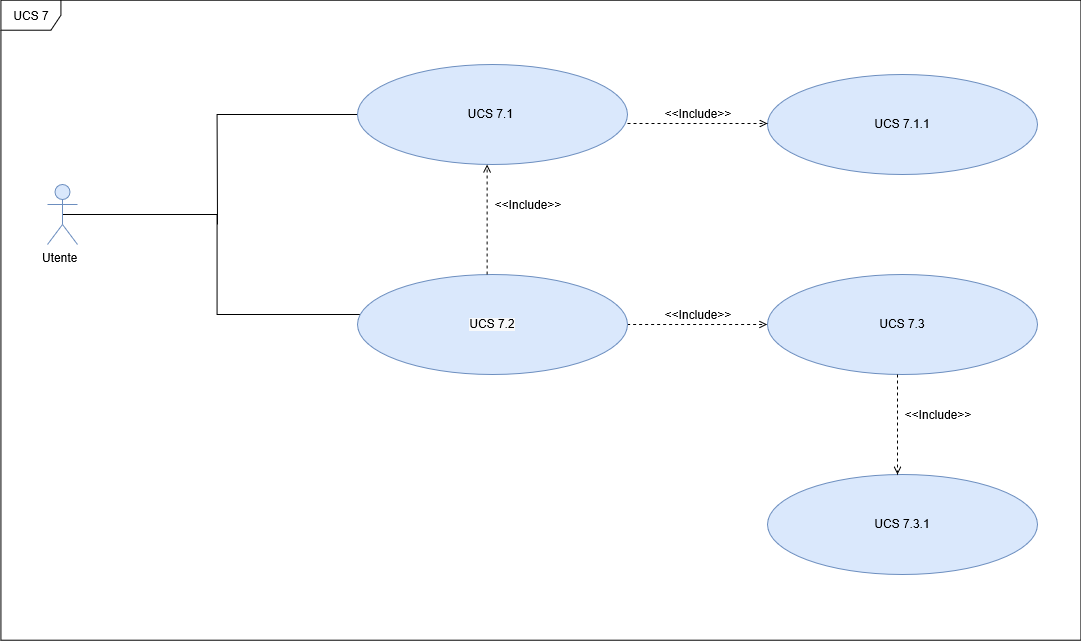
\includegraphics[scale=0.3]{sezioni/UseCase/Immagini/UCS7.png}
	\caption{Visualizzazione della lista degli accessi di un utente riconosciuto}
\end{figure}

\begin{itemize}
\item \textbf{Attori primari:} Amministratore visualizzatore;
\item \textbf{Precondizione:} L’amministratore deve essere autenticato\ap{G} presso il sistema e deve aver selezionato un'organizzazione;
\item \textbf{Postcondizione:} L’amministratore avrà visualizzato una lista di tutti gli utenti riconosciuti presenti nell'organizzazione scelta e, se vuole fare una ricerca più dettagliata, potrà selezionare la funzionalità di visualizzazione degli accessi in base a una data;
\item \textbf{Scenario principale:} L’amministratore, dopo aver selezionato l'organizzazione, accede alla funzionalità di visualizzazione della lista degli accessi di un utente riconosciuto per poter visualizzare la sua lista degli accessi;
\item \textbf{Flusso di eventi:} 
\begin{enumerate}
	\item UCS 3 l'amministratore ha selezionato l'organizzazione;
	\item L'amministrazione deve selezionare la funzionalità di visualizzazione della lista degli accessi;
\end{enumerate}
\item \textbf{Estensioni:} Visualizzazione di un messaggio che informa l’indisponibilità del server [?????];
\item \textbf{Inclusioni:}
\begin{enumerate}
	\item UCS 3 l'amministratore ha selezionato l'organizzazione.
\end{enumerate}
\end{itemize}

\subsubsection{UC 7.1 - Visualizzazione della lista con tutti gli utenti riconosciuti }
\begin{itemize}
	\item \textbf{Attori primari:} Amministratore visualizzatore;
	\item \textbf{Precondizione:} L'amministratore si trova nella sezione di visualizzazione della lista degli accessi di un utente riconosciuto (UCS 7);
	\item \textbf{Postcondizione:} L'amministratore può selezionare un'utente riconosciuto;
	\item \textbf{Scenario principale:} L'amministratore deve aver scelto la funzionalità di visualizzazione della lista degli accessi di un utente riconosciuto per poter visualizzare tutti gli utenti riconosciuti presenti nell'organizzazione precedentemente selezionataa;
	\item \textbf{Flusso di eventi:} 
	\begin{enumerate}
		\item l'amministratore visualizzza tutti gli utenti riconosciuti presenti all'interno dell'organizzazione;
		\item UCS 7.2 l'amministratore selezionerà un'utente riconosciuto;
	\end{enumerate}
	\item \textbf{Inclusioni:}
	\begin{enumerate}
		\item UCS 7.2;
	\end{enumerate}
\end{itemize}

\subsubsection{UC 7.2 - Selezione dell'utente riconosciuto }
\begin{itemize}
\item \textbf{Attori primari:} Amministratore visualizzatore;
\item \textbf{Precondizione:} L'amministratore ha visualizzato una lista con tutti gli utenti riconosciuti presenti all'interno dell'organizzazione (UCS 7.1);
\item \textbf{Postcondizione:} L'amministratore visualizzerà la lista degli accessi dell'utente riconosciuto selezionato;
\item \textbf{Scenario principale:} L'amministratore deve selezionare l'utente riconosciuto dalla lista di tutti gli utenti per poter visualizzare la sua lista degli accessi;
\item \textbf{Flusso di eventi:} 
	\begin{enumerate}
		\item l'amministratore seleziona un'utente riconosciuto dalla lista di tutti gli utenti riconosciuti presenti all'interno dell'organizzazione;
		\item UCS 7.3 l'amministratore visualizzerà tutti gli accessi dell'utente selezionato;
	\end{enumerate}
	\item \textbf{Inclusioni:}
	\begin{enumerate}
		\item UCS 7.3;
	\end{enumerate}
\end{itemize}

\subsubsection{UC 7.3 - Visualizzazione degli accessi di un'utente riconosciuto }
\begin{itemize}
	\item \textbf{Attori primari:} Amministratore visualizzatore;
	\item \textbf{Precondizione:} L'amministratore ha selezionato un'utente riconosciuto (UCS 7.2);
	\item \textbf{Postcondizione:} L'amministratore avrà visualizzato una lista con gli accessi dell'utente riconosciuto selezionato e se vuole potrà approfondire la ricerca selezionando la funzionalità di visualizzazione degli accessi in base a una data (UCS 7.4);
	\item \textbf{Scenario principale:} L'amministratore ha visualizzato la lista degli accessi delll'utente riconosciuto selezionato;
	\item \textbf{Flusso di eventi:} 
	\begin{enumerate}
		\item l'amministratore visualizzerà la lista di tutti dell'utente riconosciuto;
		\item UCS 7.4 l'amministratore, se vuole, potrà selezionare la funzionalità di visualizzazione degli accessi in base a una data;
	\end{enumerate}
\end{itemize}


\begin{figure}[h]
	\centering
	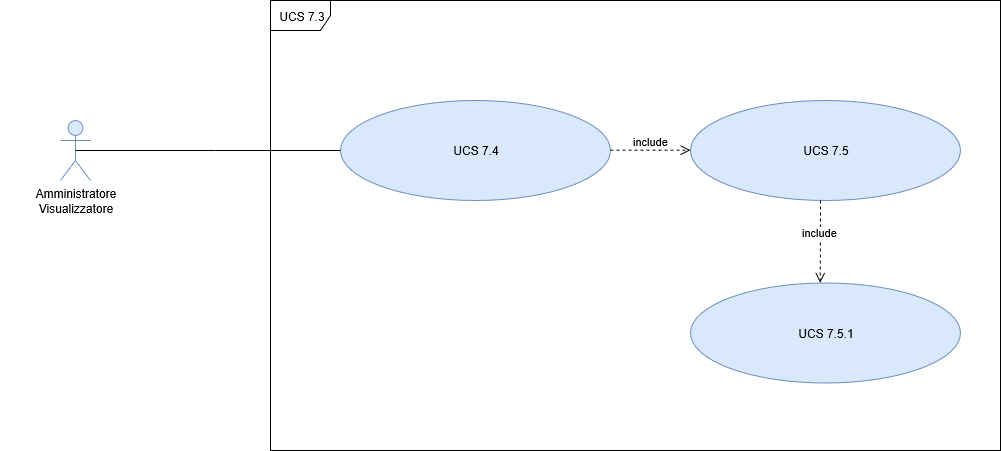
\includegraphics[scale=0.3]{sezioni/UseCase/Immagini/UCS7_1.png}
	\caption{Funzionalità di visualizzazione degli accessi in base a una data }
\end{figure}


\subsubsection{UC 7.4 - Selezione della funzionalità di visualizzazione degli accessi in base a una data }
\begin{itemize}
	\item \textbf{Attori primari:} Amministratore visualizzatore;
	\item \textbf{Precondizione:} L'amministratore avrà visualizzato tutti gli accessi dell'utente riconosciuto selezionato in precedenza (UCS 7.3);
	\item \textbf{Postcondizione:} L'amministratore potrà inserire la data per poter restringere la ricerca degli accessi (UCS 7.5);
	\item \textbf{Scenario principale:} L'amministratore, dopo aver selezionato la funzionalità di visualizzazione degli accessi in base a una data, potrà inserire una data per ottenere una ricerca più dettagliata degli accessi dell'utente riconosciuto;
	\item \textbf{Flusso di eventi:} 
	\begin{enumerate}
		\item l'amministratore ha scelto la funzionalità di visualizzazione degli accessi in base a una data;
		\item UCS 7.5 l'amministratore inserirà una data;
	\end{enumerate}
	\item \textbf{Inclusioni:}
	\begin{enumerate}
		\item UCS 7.5.
	\end{enumerate}
\end{itemize}

\subsubsection{UC 7.5 - Inserimento della data }
\begin{itemize}
	\item \textbf{Attori primari:} Amministratore visualizzatore;
	\item \textbf{Precondizione:} L'amministratore deve aver selezionato la funzionalità di visualizzazione degli accessi in base a una data (UCS 7.4);
	\item \textbf{Postcondizione:} L'amministratore potrà inserire la data (UCS 7.5.1);
	\item \textbf{Scenario principale:} L'amministratore, dopo aver inserito una data, potrà selezionare visualizzare gli accessi dell'utente riconosciuto;
	\item \textbf{Flusso di eventi:} 
	\begin{enumerate}
		\item l'amministratore inserisce la data in cui vuole visualizzare gli accessi di un utente riconosciuto;
		\item l'amministratore visualizzerà gli accessi che corrispondono alla data inserita dell'utente riconosciuto precedentemente selezionato;
	\end{enumerate}
	\item \textbf{Inclusioni:}
	\begin{enumerate}
		\item UCS 7.5.1.
	\end{enumerate}
\end{itemize}

\subsubsection{UC 7.5.1 - Visualizzazione degli accessi in base a una data di un'utente riconosciuto }
\begin{itemize}
	\item \textbf{Attori primari:} Amministratore visualizzatore;
	\item \textbf{Precondizione:} L'amministratore deve aver inserito la data (UCS 7.5);
	\item \textbf{Postcondizione:} L'amministratore avrà visualizzato una lista con gli accessi che corrispondono alla data inserita dell'utente selezionato;
\end{itemize}


